\documentclass{article}[12pt]

\usepackage[utf8]{inputenc}
\usepackage{amsfonts,amssymb,amsmath,subfigure}
\usepackage[pdftex]{graphicx}
\usepackage{epstopdf}
\usepackage{vmargin}
\usepackage{comment}
\usepackage{tikz,multicol}

\usepackage{algorithm}
\usepackage[noend]{algpseudocode}
\usepackage{tcolorbox}

\newtcolorbox{mybox}[3][]
{
  colframe = #2!25,
  colback  = #2!10,
  coltitle = #2!20!black,  
  title    = {#3},
  #1,
}


\newcommand*\Let[2]{\State #1 $\gets$ #2}
\algrenewcommand\algorithmicrequire{\textbf{Precondition:}}
\algrenewcommand\algorithmicensure{\textbf{Postcondition:}}




\excludecomment{solution}
%\includecomment{solution}

\title{IF223 - Algorithmique distribuée\\ Rappel sur les graphes}
\date{\texttt{rfosse@labri.fr}}
\author{Rohan Fossé}
\begin{document}



\maketitle{}

\section*{Plus grande valeur}

On cherche à sélectionner cinq nombres de la liste suivante en cherchant à avoir leur somme la plus grande possible (maximiser une grandeur) et en s'interdisant de choisir deux nombres voisins (contrainte).\\

\begin{center}
  15 - 4 - 20 - 17 - 11 - 8 - 11 - 16 - 7 - 14 - 2 - 7 - 5 - 17 - 19 - 18 - 4 - 5 - 13 - 8\\  
\end{center}


Comme on souhaite avoir le plus grand résultat final, la stratégie gloutonne consiste à choisir à chaque étape le plus grand nombre possible dans les choix restants.
\begin{enumerate}
    \item Appliquez cet algorithme glouton sur le tableau;
    \item Vérifiez que {20,18,17,16,15} est une autre solution possible.
    \item Que dire de la solution gloutonne ?
\end{enumerate}


\section*{Le parc d'attraction}
    
Vous visitez un parc d'attractions proposant des spectacles à différents horaires. Voici les horaires des différents spectacles :

\begin{table}[h!]
\begin{tabular}{|c|c|c|c|c|c|c|c}
\hline
\textbf{spectacle} & \textbf{A} & \textbf{B}  & \textbf{C} & \textbf{D} & \textbf{E} & \textbf{F} & \textbf{G} \\ \hline
\textbf{horaire}   & 10h-11h    & 10h30-11h30 & 11h-12h30  & 11h30-12h  & 12h-13h    & 13h-15h    & 13h30-14h  \\ \hline
\end{tabular}
\end{table}

\begin{table}[h!]
\centering
\begin{tabular}{l|l|l|}
\hline
\textbf{H} & \textbf{I} & \textbf{J} \\ \hline
14h-15h30  & 15h-16h    & 16h-17h30  \\ \hline
\end{tabular}
\end{table}

Vous avez remarqué qu'il n'est pas possible d'assister à tous les spectacles puisque certains ont lieu à des moments communs. Vous souhaitez assister à un maximum de spectacles sur la journée. Quels spectacles devez-vous choisir ?

    \begin{enumerate}
        \item Trouvez deux algorithmes gloutons pour ce problème
        \item Appliquez ces deux stratégies au problème.
        \item Laquelle donne la meilleure solution ?
    \end{enumerate}
    
\section*{Bipartition}
Étant donné un ensemble de n nombres, répartissez les en 2 sous-ensembles tels que la somme des éléments du premier soit égal à la somme des éléments du second. Proposez des algorithmes gloutons pour résoudre ce problème. Appliquez les aux ensembles suivants :
\begin{center}
   \{2, 10, 3, 8, 5, 7, 9, 5, 3, 2\}\\
\{771, 121, 281, 854, 885, 734, 486, 1003, 83, 62\} 
\end{center}

\section*{Arbres non-isomorphes}
Donner tous les arbres non-isomorphes à :
\begin{enumerate}
    \item 1, 2 ou 3 sommets
    \item 4 sommets
\end{enumerate}

\section*{Arbres couvrants}

Soit G = (S, A) un graphe non orienté (pas forcément connexe). on appelle forêt couvrante maximale tout sous-graphe de G couvrant, sans cycle, et telle que l'ajout d'une arête quelconque crée un cycle.

\begin{enumerate}
    \item Montrer que si G est connexe, toute forêt couvrante maximale est un arbre couvrant.
    \item Montrer que si le nombre d'arêtes d'une forêt couvrante est $|S|$ - k où k est le nombre de composantes connexes de G.
\end{enumerate}

\section*{Algorithme de Prim}

Appliquer l'algorithme de Prim pour trouver un arbre couvrant de poids minimum du graphe G représenté sur la figure ci-dessous.

\begin{figure}[h!]
    \centering
    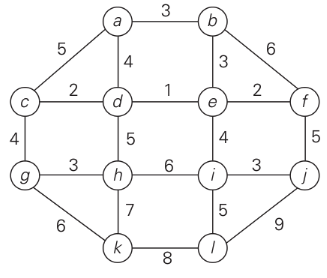
\includegraphics[scale=0.8]{Prim-1.png}
    \label{fig:my_label}
\end{figure}

\end{document}